  Dieses Kapitel behandelt die Evaluation der Java Web Frameworks. Es werden die
  Methoden zur Entscheidungsfindung bei einer Evaluation angewendet. Mit der
  definition von sinnvollen Rahmenbedingungen soll die Evaluation durchgeführt
  und die Resultate vorgelegt werden.
    
  \section{Rahmenbedingungen für die Evaluierung}
  
  Die Rahmenbedingungen für die Evaluierung werden über Soll-Kriterien und
  KO-Kriterien festgelegt.

  \subsection{Soll-Kriterien}
  
  Die Eignung, der zu evaluierenden Java Web Frameworks, wird durch eine Menge
  von Soll-Kriterien bestimmt. Die Soll-Kriterien bestimmen die Anforderungen,
  welche erfüllt werden sollen. Die Anforderungen stammen von einer
  Projektgruppe der Hochschule für Technik und Wirtschaft Berlin. Die
  Soll-Kriterien werden für den Einsatz in der \ac{ZKB} priorisiert.
  
  Soll-Kriterien sind Vorgaben, die möglichst weitgehend Erfüllt werden sollen.
  Wenn ein solches Kriterium nicht erfüllt werden kann, schliesst das die
  Alternative nicht aus. Jedem Soll-Kriterium wird für die Identifikation eine
  eindeutige ID vergeben. Die ID setzt sich folgendermassen zusammen: 
  \{Soll\}-\{Laufnummer\}.
  
  \subsubsection{Anforderungen an Web Frameworks nach AgileLearn}
  
  Eine Projektgruppe namens AgileLearn von der Hochschule für Technik und
  Wirtschaft Berlin befasst sich mit dem Thema Web Frameworks. Die
  Projektgruppe hat sich die Frage gestellt: ``\begin{itshape}Welche
  Anforderungen müssen bei der Wahl eines Webframeworks berücksichtigt
  werden?\end{itshape}''\footnote{Zitat von Raoul Jaeckel, siehe
  \cite{AnforderungenAnWebframeworks}}. Aus der Fragestellung heraus, haben sie
  18 Anforderungen an ein Web Framework ausgearbeitet, welche öffentlich in
  einem Google-Doc\footnote{Ein Service von Google um Dokumente öffentlich zu
  bearbeiten.} ersichtlich sind.
  
  Folgende Anforderungen stammen aus dem Dokument ``\begin{itshape}18
  Anforderungen an Webframeworks -
  OpenDoc\end{itshape}'', siehe \cite{AnforderungenAnWebframeworks}, und werden
  im Anhang \ref{chapter:18AnforderungenNachAgileLearn}
  \nameref{chapter:18AnforderungenNachAgileLearn} S.
  \pageref{chapter:18AnforderungenNachAgileLearn}ff zusammengefasst und mit
  einer ID versehen.

  \subsection{KO-Kriterien}
  
  Anhand einer Menge von KO-Kriterien wird die Auswahl der Alternativen
  eingeschränkt. Die KO-Kriterien sind aus dem \begin{itshape}Handbuch der
  IT-Architektur\end{itshape}, siehe \cite{ZkbHandbuchDerItArchitektur}, der
  \ac{ZKB} entnommen. Die Namensgebung in dem Handbuch unterscheidet sich
  leicht, es wird nicht von KO-Kriterien, sondern von Grundsätzen gesprochen.
  
  KO-Kriterien sind Vorgaben, welche zwingend erfüllt sein müssen. Falls ein
  Kriterium nicht erfüllt werden kann, fällt die Entscheidung auf diese
  Alternative negativ aus. Jedem KO-Kriterium wird für die Identifikation eine
  eindeutige ID vergeben. Die ID setzt sich folgendermassen zusammen: 
  \{KO\}-\{Laufnummer\}.

  \subsubsection{Grundsätze aus der IT-Architektur der Zürcher Kantonalbank}
  
  Ein Grundsatz wird im Handbuch wer IT-Architektur wie folgt definiert:\\
  
  ``\begin{itshape}Es sind Grundsätze definiert, nach denen sich die Baupläne
  der IT-Systeme zu richten haben. Die Grundsätze sind ein Regelwerk mit
  Weisungscharakter.\end{itshape}''
  \footnote{\cite{ZkbHandbuchDerItArchitektur} Kapitel 1.3 - \begin{itshape}Was
  ist die IT-Architektur der ZKB\end{itshape}, Seite 11}
  \\
  \\
  \noindent
  Dabei gibt es eine Hintertür:\\

  ``\begin{itshape}Grundsätze sind verbindliche Vorgaben (Konventionen), von
  denen nur in begründeten Ausnahmen abgewichen werden kann.\end{itshape}''
  \footnote{\cite{ZkbHandbuchDerItArchitektur} Kapitel 1.8 -
  \begin{itshape}Leseanleitung\end{itshape}, Seite 14}
  \\
  \\
  \noindent
  Das Dokument wurde analysiert und alle Grundsätze, welche für diese
  Diplomarbeit relevanten sind, werden im Anhang
  \ref{chapter:GrundsaetzeDerZkbItArchitektur}
  \nameref{chapter:GrundsaetzeDerZkbItArchitektur} auf S.
  \pageref{chapter:GrundsaetzeDerZkbItArchitektur}ff aufgelistet und mit einer
  ID versehen.

  \section{Hirarchie der Soll-Kriterien}
  
  Da 18 Soll-Kriterien definiert wurden und diese in jeder Alternative 
  untersucht werden müssten, würde das den Rahmen der Diplomarbeit sprengen.
  Desshalb sollen die Soll-Kriterien in eine Hirarchie entsprechend ihrer
  Wichtigkeit für die \ac{ZKB} aufgeteilt werden. Die Hirarchie wird in zwei
  Gruppen aufgeteilt:
  
  \begin{itemize}
    \item wichtig
    \item nicht wichtig
  \end{itemize}
  
  \subsection{Priorisierung für die ZKB}
  
  Wichtige Aspekte für die \ac{ZKB} im Software-Lebenszyklus sind:
  
  \begin{description}
    \item[Sicherheit]
    Nur eine Bank, die als sicher gilt, hat das Vertrauen der Kunden und somit
    Erfolg in ihrem Geschäft.
    \item[Kosten]
    Die laufenden Kosten sollen so tief wie möglich gehalten werden. Gemäss
    Abbildung \ref{img:softwareLifecycleCost} liegen die Hauptkosten im
    Software-Lebenszyklus bei der Maintenance-Phase.
    \item[Verfügbarkeit von Ressourcen]
    Damit Software entwickelt und gewartet werden kann, werden qualifizierte
    Ressourcen benötigt.
    \item[Image]
    Um sich von der Konkurenz abzuheben wird ein Image aufgebaut das sich
    zeitgemäss präsentieren soll.
  \end{description}
  
  \begin{figure}[ht]
    \begin{center}
      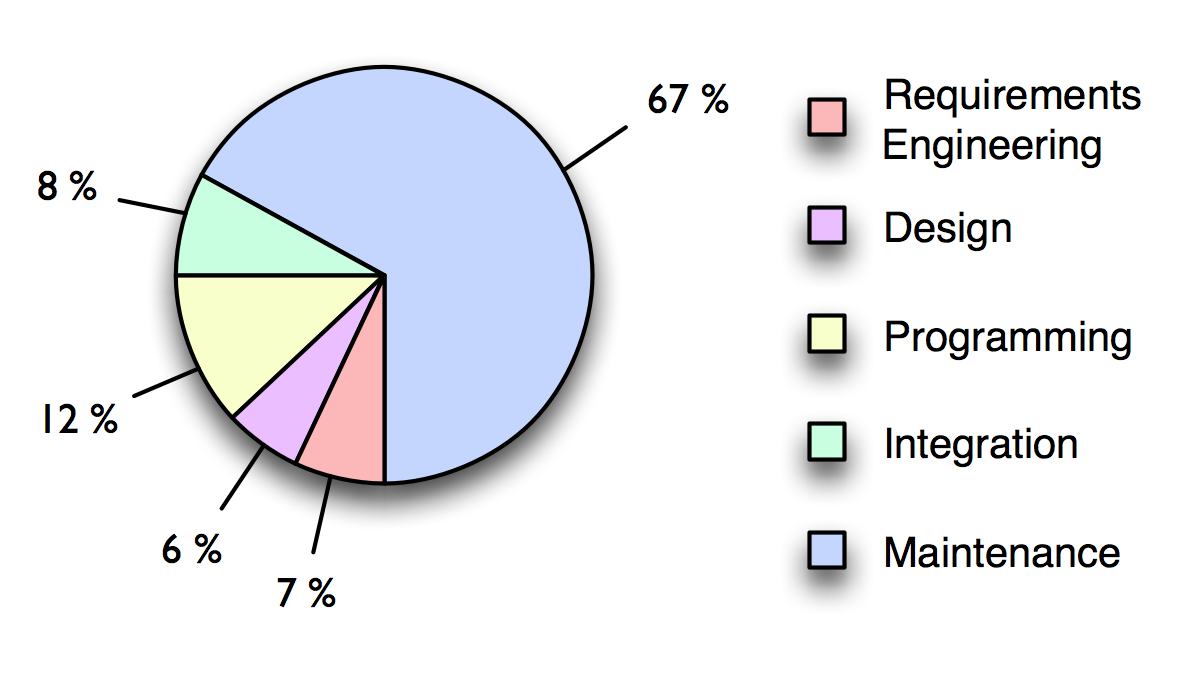
\includegraphics[width=0.85\textwidth]{./image/softwareLifeCycleCost.png}
      \caption{Ungefähre relative Kosten der Phasen des Software-Lebenszyklus
      (nach \cite{SoftwareEngineering} S. 11 und
      \cite{SoftwareLifeCycleModels})}
      \label{img:softwareLifecycleCost}
    \end{center}
  \end{figure}
  
  
  ``MVC-Entwurfsmuster''
  \newline
  \newline
  \noindent
  Das MVC-Konzept ist sicher gut, sollte aber nicht eine Anforderung an ein Web
  Framework sein, da es viele ebenbürdige Alternativen gibt.
  \newline
  
  ``Object Relational Mapping (ORM)''
  \newline
  \newline
  \noindent
  In der Java Welt gibt es viele ORM Lösungen, welche sich in den Jahren
  durchgesetzt haben, ein paar nennenswerte sind Hibernate, TopLink und
  EclipseLink. Diese Anforderung entfällt also.
  \newline
  
  Folgende Punkte wurden in den Katalog der Soll-Kriterien aufgenommen und somit
  mit einer eindeutigen ID versehen:
  
  \section{Auswahl der Java Web Frameworks}
  
  Es sollen vier Java Web Frameworks für die Evaluation ausgewählt werden. Ein
  Java Web Framework, das in Frage kommt, wird Alternative genannt.
  
  \subsection{Begründung}
  
  \subsection{Prüfen auf bestehende KO-Kriterien}
  
  \section{Gewichtete Nutzwertanalyse mit dem Analytic Hirarchy Process}
  
  \subsection{Bestimmen der Kriterien}
  
  \subsection{Bestimmen der Gewichte mit dem Analytic Hirarchy Process}
  
  \subsection{Bestimmen des Erfüllungsgrads}
  
  \section{Resultat}
